\documentclass[conference]{IEEEtran}
\IEEEoverridecommandlockouts
% The preceding line is only needed to identify funding in the first footnote. If that is unneeded, please comment it out.
\usepackage{cite}
\usepackage{url}
\usepackage{seqsplit}
\usepackage{caption}
\usepackage{subcaption}
\usepackage{amsmath,amssymb,amsfonts}
\usepackage{graphicx}
\usepackage{textcomp}
\usepackage{xcolor}
\usepackage{kotex}
\usepackage{multicol}
\usepackage{multirow}
\usepackage{booktabs} % For better-looking tables
\usepackage{makecell}
\usepackage{algorithm}
\usepackage{algpseudocode}
\def\BibTeX{{\rm B\kern-.05em{\sc i\kern-.025em b}\kern-.08em
    T\kern-.1667em\lower.7ex\hbox{E}\kern-.125emX}}
\begin{document}

\title{Upstream Based Low Latency Auto-scaling For Microservices *\\}

\author{\IEEEauthorblockN{%1\textsuperscript{st} 
    Jaehong Lee, and Euiseong Seo}
\IEEEauthorblockA{\textit{Department of Software, Sungkyunkwan University} \\
% \textit{name of organization (of Aff.)}\\
Suwon, Republic of Korea \\
{\{tutu083, euiseong\}@skku.edu}
}
}

\maketitle


% ----------------------------------------------------------------------------



\begin{abstract}

    scalability는 마이크로서비스 아키텍에서 중요한 ability중 하나이다
    마이크로서비스 오케스트레이션을 위한 the de-factor standard인 쿠버네티스는 HPA라는 auto scaling 기능을 제공한다. 하지만 hpa의 polling 메커니즘은 ms가 스케링이 되는 동안 발생하는 interval에 의해 전체 클러스터 성능 및 서비스 품질 저하 및 realtime에 활용 되기 역부족
    본 논문에서는 polling 구조를 개선한 upstream 기반 auto scaling 제안
    DeathStarBench를 통한 성능 평가
    우리의 접근 방식은 성능 향상과 함께 무시할 만한 정도의 리소스 사용했음

\end{abstract}


% ----------------------------------------------------------------------------


\begin{IEEEkeywords}
    microservices, auto-scaling, kubernetes, resource management
\end{IEEEkeywords}


% ----------------------------------------------------------------------------


\section{Introduction}
Scalability of Microservices and Kubernetes.
마이크로서비스 아키텍처는 서비스 운영 효율을 높이기 위한 패러다임으로 자리 잡았다. 최근 대규모 서비스들의 운영 및 관리 효율을 위한 주요 패러다임으로 자리잡은 후 각 서비스들의 요구사항에 맞춰 지속적으로 고도화 되고있다. 기존 모놀리식 기반 아키텍처와 달리 마이크로서비스 아키텍처는 각 마이크로서비스들의 자원을 독립적으로 스케일링 하여 효율적인 자원 관리가 가능하다. 마이크로 서비스 아키텍처는 하나의 애플리케이션을 잘 정의된 기능 및 서비스로 분할한다. 필요에 따라 특정 서비스만 배포하거나 확장이 가능함으로 클러스터 자원을 효율적으로 활용함과 동시에 시스템의 중단 없이 서비스를 업데이트할 수 있다. 마이크로서비스 아키텍처 구성을 위해 컨테이너들을 효율적으로 배포하고 관리하는 오케스트레이션 도구 중 CNCF의 주력 프로젝트인 쿠버네티스...

Limitation of Kubernetes Auto Scaling.
쿠버네티스는 HPA(Horizontal Pod Autoscaler) 기능을 제공한다[4].
HPA는 임계값을 기준으로 한 규칙 기반 자동 스케일링 방법으로 HPA 컨트롤러는 현재 동작중인 Pod들의 메트릭스 값과 운영자가 지정한 목표 메트릭스 값을 통해 현재 필요한 Pod의 개수를 계산 후 스케일링을 진행한다. 하지만 HPA는 각 Pod별로 메트릭스를 수집하고 반응하기까지 오랜 시간이 걸리는 문제로 급격한 트래픽 변동에 즉각적으로 대응하지 못하는 한계가 있다. 리얼 타임 시스템(TELCO, MEDIA, GAMING, FINANCE 등)에서 마이크로서비스 아키텍처 활용이 증가하고 있다.쿠버네티스 HPA의 performance는 리얼 타임 시스템에서 활용하기에 역부족하다.

Other proposals.
작성1. 실시간으로 트래픽을 예측하여 필요한 인스턴스 수를 미리 확장하는 방법[5], [6], [7]이 제안되었으나 지속적인 학습 비용과 학습된 트래픽 패턴이 아닌 경우 제한된 성능을 보여준다. 수평 스케일링과 수직 스케일링을 필요에 따라 적절히 조합하여 활용하는 하이브리드 방식[5, 8]도 제안되었다. 하지만 변동성이 심한 워크로드를 대응 하기에 한계가 있다. 다양한 metric을 활용하는 방법이 제안되었으나 보편적으로 활용 가능한 실용적인 방법은 아님

작성2. prediction에 기반한 다른 제안들이 있지만 common한 솔루션이 아니고 실제로 practical하지 못함
또한 meta 논문의 의하면 복잡한 ms 관계를 간단히 정의 또는 공식화 할 수 없음
음으로 cpu 메모리외에 다른 리소스를 활용하는 방버빙 있으나, common하지 못하고, socc 22에 나온 논문에 의하면 cpu와 메모리의 의존도가 높음 특히 그래프에서 보여주듯 cpu가 memory보다 더 중요하며 scale의 주요 타겟은 stateless이므로 cpu가 중요

Our proposal.
무시할 만한 리소스 사용으로 성능을 최적화할 수 있는 upstream 방법
cpu를 메트릭으로 활용하는 lightweigh하면서 practical한 솔루션인 UHPA를 제안

Short Conclusion.
UHPA는 HPA 대비 평균 최대 30\% 성능 향상을 보여줬고 realtime system에서 활용가능한 수준임을 보여주었다.

% ----------------------------------------------------------------------------


\section{Background and Motivation}
In cloud computing, scalability is one of the key features that enhances Quality of Service (QoS) and contributes to the success of microservice architecture. Threshold-based auto-scaling is popular for its simplicity and easy of use. https://www.overleaf.com/project/65cf81e31dd3fa18fce1b56d

\subsection{Horizontal Pod Auto Scaling of Kubernetes}
Kubernetes is a flagship project of the Cloud Native Computing Foundation(CNCF) and it is the industry standard of container orchestrator which  provides many powerful functions for flexible and efficient service operations. The Horizontal Pod Autoscaler(HPA) is a feature to automatically scale microservice application on Kubernetes. Fig. \ref{fig:hpa system design}  shows the system architecture implemented in Kubernetes along with the HPA workflow.


\begin{figure}[ht]
    \centerline{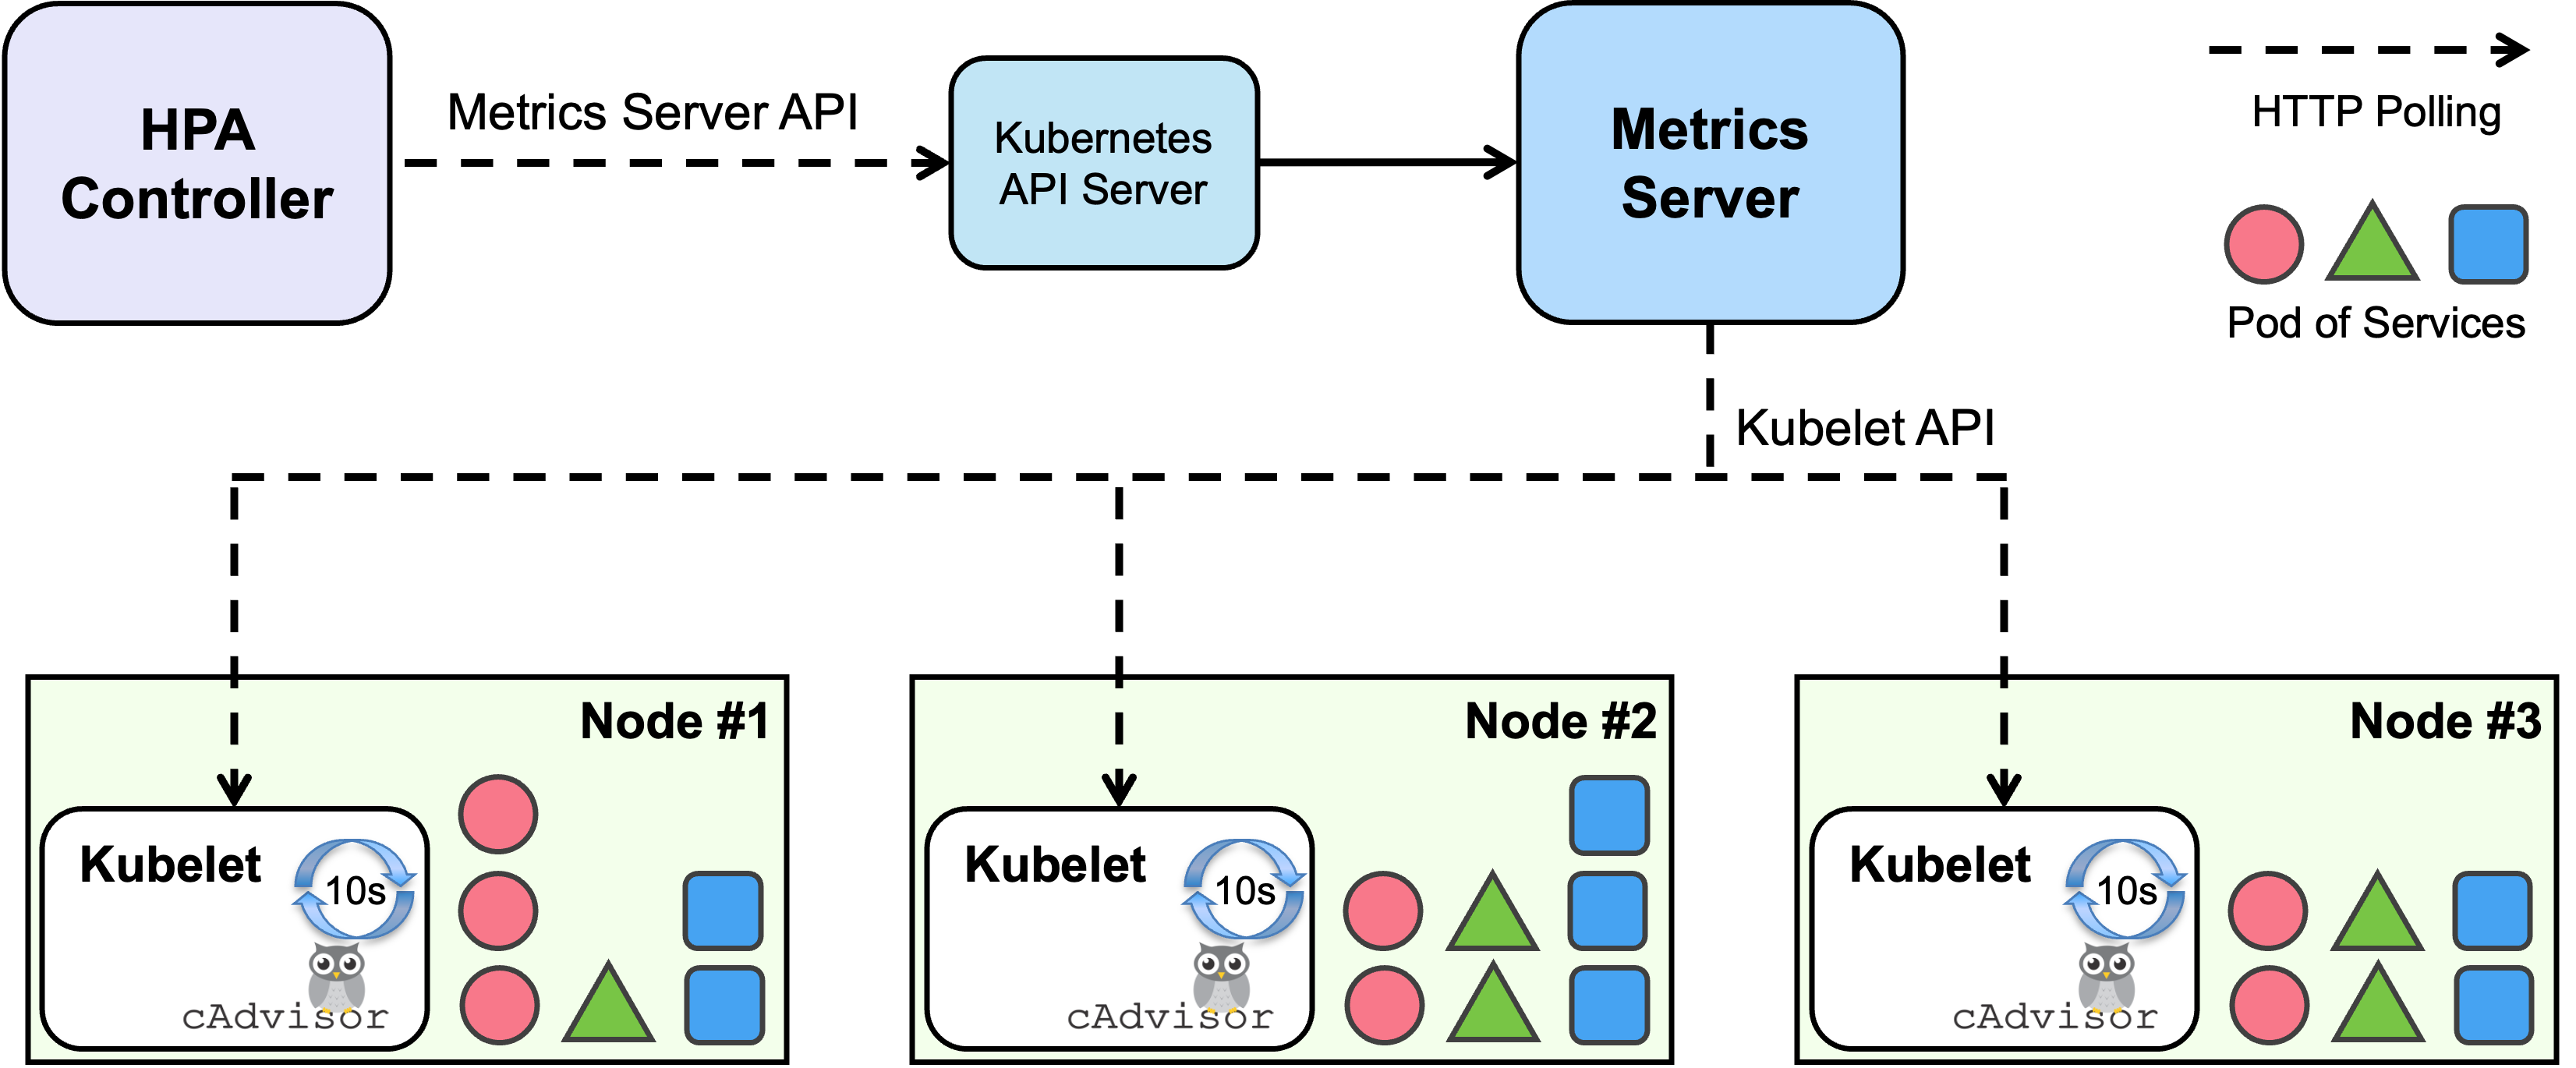
\includegraphics[width=8.5cm]{leejaehong/images/background/k8s_system_design.png}}
    \caption{HPA Workflow}
    \label{fig:hpa system design}
\end{figure}


HPA monitors the CPU usage of all the interested pods, which are the smallest units in Kubernetes, and each pod comprises a set of containers. The process of collecting metrics involves three main components: Kubelet, Metrics-server, and HPA Controller. Each component employs a polling mechanism to gather CPU usage. Initially, the Kubelet collects all raw metrics from cAdvisor at the beginning of the workflow. Subsequently, Metrics-server retrieves these metrics via the Kubelet’s REST API and expose them through the Kubernetes API server. Finally, HPA controller requests the CPU usage data from the API server.


\begin{equation}
    {\lceil Current Replicas\ast \left ( \frac{ Total CPU usage}{Target CPU usage} \right ) \rceil }
    \label{eq:HPA desired replicas}
\end{equation}

During the collection process, HPA controller determines the desired number of replicas based on the current CPU usage rate of the Pods, which are comprised of each microservice. It then scales the microservice up or down when resource usage hits a threshold\cite{KubernetesHPA}. Eq. \ref{eq:HPA desired replicas} displays the formula used by the HPA controller to calculate the required number of Pods. For instance, if a microservice with two Pods has a target CPU usage of 80\% but the actual average CPU usage is 100\%, an additional pod is automatically added to reduce the CPU usage to approximately 66.6\%.”


\subsection{Limitation of HPA}

Through the diverse experiments of HPA and an in-depth analysis of the source code of its three components, we found out that the polling mechanism exhibits a lack of reliability due to scaling delays. Especially, the default policy is not timely and causes low QoS in the high concurrency usage scenarios\cite{huo2023high}.


\begin{table}[ht!]
    \caption{Polling Interval Time of Each Component}
    \begin{center}
        \begin{tabular}{|c|c|c|}
            \hline
            \cline{2-3}
            \textbf{Component} & \textbf{{Default(s)}} & {\textbf{Optimal(s)}} \\
            \hline
            Kubelet            & 10                    & 10                    \\
            \hline
            Metrics-server     & 60                    & 15                    \\
            \hline
            HPA Controller     & 15                    & 1                     \\
            \hline
        \end{tabular}
        \label{tab:Polling Interval Time of Each Component}
    \end{center}
\end{table}


We measured the scaling performance by altering the polling interval times of HPA shown in the Table. \ref{tab:Polling Interval Time of Each Component}. Kubelet, which includes cAdvisor for collecting CPU-related metrics from the cgroup, sets the polling interval time, "housekeeping\_interval", to 10 seconds by default. Since this value is non-configurable, the interval was maintained across all experimental scenarios. Metrics-server, fetching metrics from each node's kubelet via HTTP request, collects data every 60 seconds by default. This interval can be adjusted by modifying the "metric-resolution" parameter. In optimal mode, we utilized a minimum value of 15 seconds which is recommended in the official documentation\cite{metrics-server-FAQ}. For the HPA controller, 15 seconds was used as the default interval value, and the experiment was conducted using 1 second in optimal mode.


\begin{figure}[ht!]
    \centering{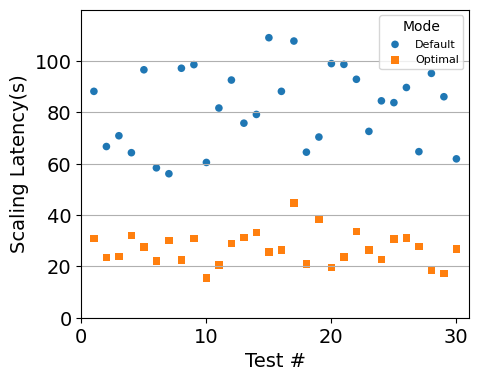
\includegraphics[width=5.7cm]{leejaehong/images/background/scaling_latency_without_UHPA.png}}
    \centering{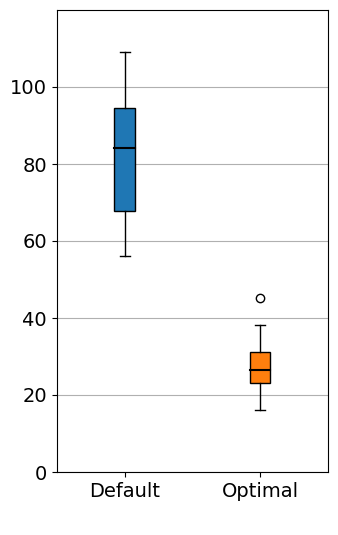
\includegraphics[width=2.8cm]{leejaehong/images/background/scaling_latency_boxplot_without_UHPA.png}}
    \caption{Scaling delay according to polling interval time}
    \label{fig:scaling time}
\end{figure}

Fig. \ref{fig:scaling time} illustrates the time taken from when the actual threshold was exceeded until the pod actually expanded in each mode. In the default mode, the results indicate a wide distribution ranging from 56 seconds to 109 seconds, with scaling being completed in approximately 82 seconds on average. On the other hand, In optimal mode, scaling occurred within an average duration of about 27 seconds, displaying a variance from 16 to 45 seconds. By Analizing of the experiment result, we were able to found two factors associated with the performance limitations of HPA.

\begin{enumerate}
    \item \textbf{Optimizing the interval time still results in significant scaling latency.} In our experiment on fine-tuning the polling interval time, we discovered that even the optimal setting for collecting metrics still has a considerable delay time. Although we saw an impressive performance improvement of nearly 70\% in optimal mode comparing to default mode, this improved setup still ended up taking around 27 seconds on average, which is quite slow. Furthermore, the Metrics-server calculates the current CPU usage by averaging both previous and latest metric values and relays this information to the HPA controller. As a result, if the load grows linearly or steeply, this averaging method will underestimate of actual CPU usage even if it exceeds the target threshold. For this reason, it shows a longer delay time than the worst case, which is the sum of all polling interval times theoretically. For example, in Fig. \ref{fig:scaling time}, most of the delay times are higher than 26 seconds, which is the sum of each polling interval time in optimal mode(10s, 15s, and 1s)

    \item \textbf{The multiple polling architecture between components is inefficient for clusters.} Through our experiments, we have found that reducing the polling interval can quite improve scaling latency. However, adjusting the reduced polling interval time will cause the Metrics-server to continuously send HTTP requests to the Kubelet on all nodes. Also, short polling interval of the HPA controller, which requests CPU usage metrics from the Metrics-server through the Kubernetes API server, causes increased load on the API server. As a result, the load on the API server increases and cluster performance can degrade due to this constant network traffic\cite{ExpediaGroupTech2020}. Moreover, This case wastes a lot of cluster resources to scrape useless metrics when scaling is not needed.
\end{enumerate}


\subsection{Related Work}
We looked into the issues and limitations of auto-scaling provided by Kubernetes.  Similarly, various methods have been proposed to analyze the problem and enhance scaling performance. These strategies show better scaling performance by solving the problems as each analyzed.

Adjusting the frequency of metric collection based on the low, medium and high workload status of the microservices has been suggested\cite{jiang2021fine}. This method provides a fine-grained auto-scaling function by changing the polling interval time according to the characteristics of the workload. However, this approach still does not overcome the limitation of the optimal setting of HPA.

Methods to predict and dynamically respond to incoming workloads have also been proposed. Using statistical models such as ARIMA show decent performance at forecasting regular workloads and  guarantee high Quality of Service by preemptive scaling based on the prediction\cite{dimolitsas2022ahp4hpa}\cite{zhao2019research}\cite{he2020novel}. However, when workload data changes, their accuracy drops significantly, especially with fluctuate workloads\cite{yunyun2022research}.

Lastly, machine learning based workload predictions have also been actively conducted\cite{dang2021deep}\cite{gan2021sage}. Machine learning models typically perform better at forecasting workloads than time-series analysis based predictions\cite{shim2023predictive}. However, using past data for learning is difficult to use in microservice architectures that often update. In addition, actual microservice composition is much more complex than benchmarking open sources. Existing analysis methods depend on various experiment environment assumptions, which might not fully reflect the actual microservice architecture\cite{huye2023lifting}. \\


To solve this problem, we introduce a novel lightweight upstream-based horizontal pod autoscaler UHPA(Upstream Based Horizontal Pod Auto Scaler). UHPA employs a two-step decision  mechanism through UHPA Agent daemons deployed on each node and a central UHPA controller to make expedite decisions and minimize meaningless network traffic.


% multiple metrics based auto-scaling에 대한 설명
% 다음으로 cpu 메모리외에 다른 리소스를 활용하는 방버빙 있으나, common하지 못하고, socc 22에 나온 논문에 의하면 cpu와 메모리의 의존도가 높음
% 특히 SOCC 22년 논문의 그래프에서 보여주듯 cpu가 memory보다 더 중요하며 scale의 주요 타겟은 stateless이므로 cpu가 중요
% 전반적으로 이러한 접근 방법이 갖는 문제점이 무엇인지 (특정 논문을 언급해서 안된다 말고, 전반적인 이러한 접근 방법의 문제점).

% ---------------------------------------------------------------- ------------


\section{Upstream Based Horizontal Pod Auto Scaler}
\subsection{System Overview}

\begin{figure}[ht!]
    \centerline{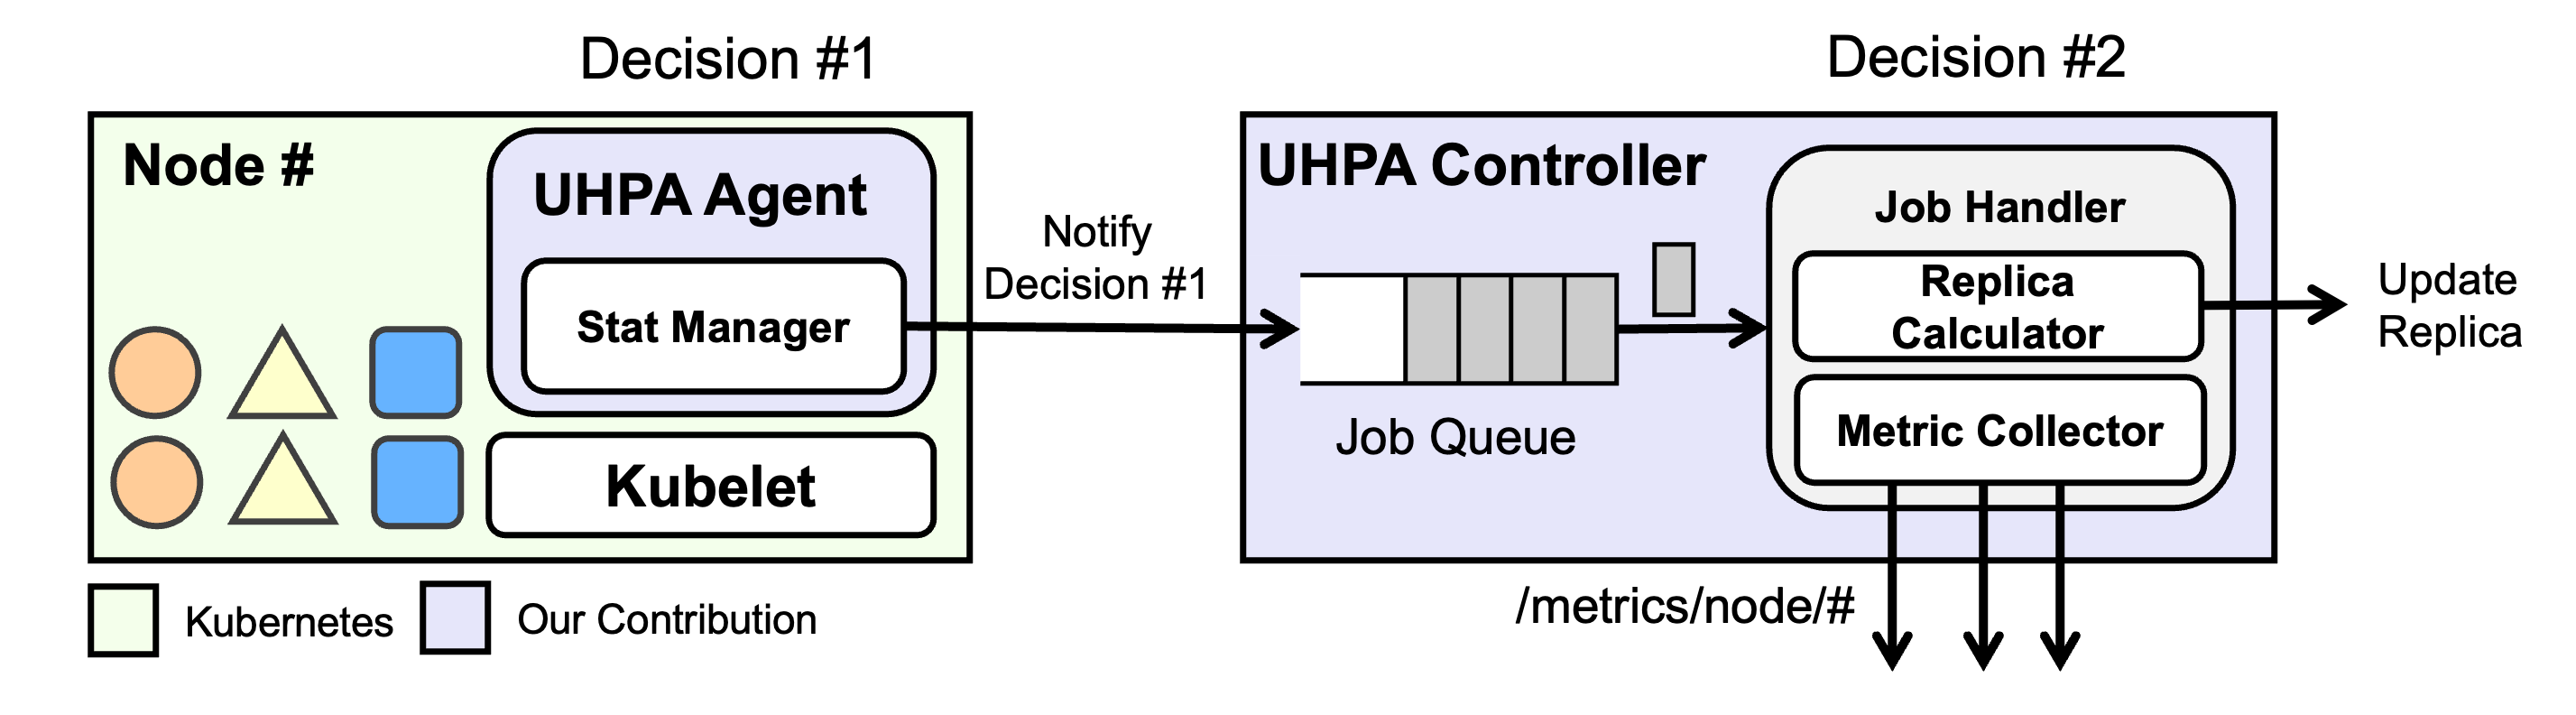
\includegraphics[width=8.5cm]{leejaehong/images/approch/uhpa_system_design.png}}
    \caption{System Overview of UHPA}
    \label{fig:uhpa system design}
\end{figure}
Fig. \ref{fig:uhpa system design} illustrates the system architecture of the Upstream based Horizontal Pod Autoscaler (UHPA), designed to enhance auto-scaling performance within a Kubernetes cluster with the two main components: the UHPA Agent and the UHPA Controller. Deployed as a Daemon across all worker nodes in the cluster, the UHPA Agent is tasked with periodically gathering pod CPU usage via the Stat Manager. Unlike the HPA’s conventional polling-based approaches for metric collection, UHPA adopts an upstream-based strategy that triggers scaling decisions preemptively by the UHPA Agents. The UHPA Agent makes a pre-decision to identify microservices  that necessitate scaling with collected CPU usage on its own node and then notifies the UHPA Controller of the results. This method significantly enhances detecting performance when thresholds are reached.

To reduce system complexity, the UHPA Agents interact exclusively with the UHPA Controller. The Controller, therefore, is responsible for collecting scaling-relevant information through the Kubernetes API Server and providing it to all UHPA Agents. The UHPA Controller manages notifications received from each UHPA Agent by organizing them into jobs, queuing these jobs, and periodically dequeuing them to ultimately decide whether to scale or not. Our approach addresses the inefficiency arising from the three-component interaction model in HPA by transitioning to the more efficient two-component model.


\subsection{Lightweight CPU Metric Collection}
We chose CPU usage as the main metric because most services within microservice architecture are stateless which is more affected by CPU usage than others. One of the most greatest advantages of microservice architecture is that they are Independently deployable, loosely-coupled\cite{MicroservicesIO} and to take advantage of these benefits, microservices are mainly stateless services which do not store and maintain any state data to simplify deployment, scaling, and replacement for scalability and reliability\cite{AWSStatefulActorServices2023}. Except for specific cases such as storage services for stable and continuous data, ordered and graceful deployment, scaling and rolling updates, the stateless service is the basic type of microservice architecture\cite{KubernetesStatefulSet2023}\cite{gan2019open}.

OS-level metrics CPU and memory usage are more highly correlated with workloads in microservice architecture than other application-level metrics\cite{luo2022power}. With tracking frameworks like Jaeger\cite{JaegerTracing}, methods that use application-level metrics, such as response time, have been proposed\cite{pramesti2022autoscaling}\cite{gan2021sage}. However, these metrics can be affected by various external system environments\cite{luo2022power}, and their limited experimental settings may not accurately represent industrial microservice architectures or request workloads\cite{huye2023lifting}. Kubernetes HPA provides a memory-based pod auto-Scaling function, but it's primarily tailored for specific services like databases and caching services that are less sensitive to scaling performance. Informed by this research, UHPA decided on CPU usage, a simple but powerful OS-level metric, as the scaling metric.

Kubelet deployed on each node collects and exports various information related to the network and disk, as well as the CPU and memory usage of all deployed containers, through the built-in cAdvisor\cite{cAdvisorGithub} to collect OS-level metrics. The housekeeping-interval, which is the basic collection scraping interval, is fixed to 10 seconds. This is because cAdvisor collects a large amount of information related to all containers running on the node, so if the scraping time is too shortened, it may result in high CPU usage\cite{KubecostcAdvisor}.

To solve the issue that high CPU usage by cAdvisor, we adopt a lightweight strategy that collects only CPU metric of microservices registered by HorizontalPodAutoscaler of Kubernetes.
\begin{enumerate}
    \item All UHPA Agents periodically obtain information on microservices registered in the HorizontalPodAutoscaler through the UHPA Controller.

    \item UHPA Agent updates information on the each container path that exists under “/sys/fs/cgroup/” with the container ID of the containers included in the pods that make up the microservices.

    \item Every second, UHPA Agent reads CPU metrics from the container path and calculates the CPU usage rate of the pod.
\end{enumerate}

We use the 5-second average data to ignore cases of abnormal spikey workloads in a very short period of time.

\subsection{Two-step Decision Mechanism}
First Decision from Agents.
1차 node, 2차 controller를 통해서 decision을 두번함 upstream 구조를 위해 1차 decision을 노드가 내림. 각 파드에 동일하게 리퀘스트가 분배되지 않기 때문에 node decision은 참고용으로 활용함
First Decision from Agent.
use average metric data
데이터 안정성을 위한 변화율 시간 메트릭 decision (이걸 Node에서 처리).
e.g. (sample(t2) - sample(t1)) / (t2 - t1)
Final Decision from Controller

\begin{algorithm}[ht!]
    \caption{First Decision Procedure in UHPA Agent}
    \begin{algorithmic}[1]
        \While{\textbf{true}}
        \State $l \gets \text{an empty list}$
        \For{\textbf{each} $int\_MS$ \textbf{in} $int\_MSs$}
        \State $tcr \gets 0$
        \For{\textbf{each} $pod$ \textbf{in} $int\_MS\rightarrow\text{pods}$}
        \State $tcr \gets t + \Call{CalCPURate}{pod}$
        \EndFor
        \State $acr \gets tcr / \Call{Length}{int\_MS\rightarrow\text{pods}}$
        \If{$acr > int\_MS\rightarrow\text{threshold}$}
        \State \Call{Append}{$l, int\_MS$}
        \EndIf
        \EndFor
        \If{$\Call{Length}{l} > 0$}
        \State \Call{NotifyToController}{$l$}
        \EndIf
        \State \Call{Sleep}{1}
        \EndWhile
        \label{alg:agent}
    \end{algorithmic}
\end{algorithm}


\begin{algorithm}[ht!]
    \caption{Final Decision Procedure in UHPA Controller}
    \begin{algorithmic}[1]
        \While{\textbf{true}}
        \State $j \gets \Call{Dequeue}{Job}$
        \State $css \gets \Call{GetCPUStatFromAllAgents}{j\rightarrow\text{MS}}$
        \State $e \gets 0$
        \State $tcr \gets 0$
        \For{\textbf{each} $cs$ \textbf{in} $css$}
        \If{\Call{IsExist}{$cr$}}
        \State $tcr \gets tcr + \Call{CalCPURate}{cs}$
        \State $e \gets e + 1$
        \EndIf
        \EndFor
        \State $acr \gets tcr / e$
        \If{$acr > j.threshold$}
        \State \Call{DoScale}{$j\rightarrow\text{MS}$}
        \EndIf
        \EndWhile
        \label{alg:controller}
    \end{algorithmic}
\end{algorithm}

...


% ----------------------------------------------------------------------------


\section{Evaluation}
\subsection{Evaluation Setup}
...

\subsection{Latency Analysis}
Time Breakdown of Performance with simple app
Fig4기존 hpa대비 얼마나 빨리 scaling되는지 보여준다

\begin{figure}[ht!]
    \centering{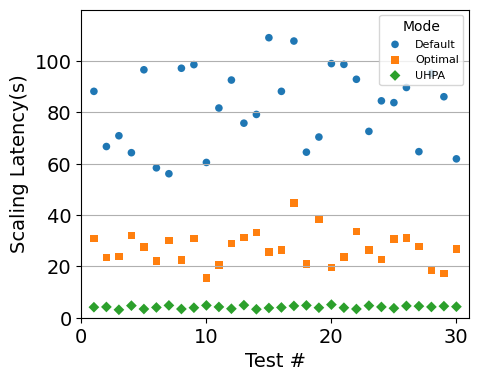
\includegraphics[width=5.7cm]{leejaehong/images/evaluation/scaling_latency_with_UHPA.png}}
    \centering{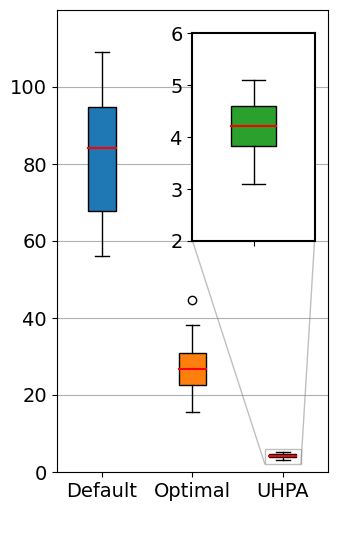
\includegraphics[width=2.8cm]{leejaehong/images/evaluation/scaling_latency_boxplot_with_UHPA.png}}
    \caption{Scaling Latency Comparison}
    \label{fig3}
\end{figure}
\begin{table}[ht!]
    \caption{Scaling Performance Comparison}
    \begin{center}
        \begin{tabular}{|c|c|c|c|}
            \hline
            \multicolumn{4}{|c|}{\textbf{Scaling Latency(s)}}                                          \\
            \cline{1-4}
            \hline
            \textbf{} & \textbf{\textit{Default}} & \textbf{\textit{Optimal}} & \textbf{\textit{UHPA}} \\
            \hline
            Average   & 81                        & 27                        & 4                      \\
            \hline
            Min       & 51                        & 16                        & 3                      \\
            \hline
            Max       & 109                       & 45                        & 5                      \\
            \hline
            Perc.95   & 108                       & 41                        & 5                      \\
            \hline
        \end{tabular}
        \label{tab:scaling_performance_comparison}
    \end{center}
\end{table}


\begin{table}[ht!]
    % \begin{subtable}[h]{0.5\textwidth}
    \centering
    \begin{tabular}{c|ccc|ccc}
        \noalign{\smallskip}\noalign{\smallskip}\hline\hline
        \multirow{2}{*}{\makecell{CPU                              \\Limit}} & \multicolumn{3}{c|}{Linear} & \multicolumn{3}{c}{Spike} \\
        \cline{2-7}
             & Default & Optimal & UHPA & Default & Optimal & UHPA \\
        \hline
        x1.0 & 22\%    & 26\%    & 34\% & 17\%    & 20\%    & 30\% \\
        x1.5 & 36\%    & 44\%    & 64\% & 28\%    & 33\%    & 48\% \\
        x2.0 & 47\%    & 64\%    & 85\% & 37\%    & 47\%    & 72\% \\
        x2.5 & 57\%    & 84\%    & 94\% & 46\%    & 68\%    & 89\% \\
        \hline
        \hline
    \end{tabular}
    \caption{Linear}
    \label{tab:success_rate_linear}
    % \end{subtable}
    % \hfill
    % \begin{subtable}[h]{0.5\textwidth}
    %     \centering
    %     \begin{tabular}{c|ccc|ccc}
    %     \noalign{\smallskip}\noalign{\smallskip}\hline\hline
    %     \multirow{2}{*}{\makecell{CPU\\Limit}} & \multicolumn{3}{c|}{Linear} & \multicolumn{3}{c}{Spike} \\
    %     \cline{2-7}
    %           & Default  & Optimal & UHPA & Default  & Optimal & UHPA  \\
    %     \hline
    %      x1.0 & 22\% & 26\% & 34\% & 22\% & 26\% & 34\% \\
    %      x1.5 & 36\% & 44\% & 64\% & 36\% & 44\% & 64\% \\
    %      x2.0 & 47\% & 64\% & 85\% & 47\% & 64\% & 85\% \\
    %      x2.5 & 57\% & 84\% & 94\% & 57\% & 84\% & 94\% \\
    %     \hline
    %     \hline
    %     \end{tabular}
    %     \caption{Spike}
    %     \label{tab:success_rate_spike}
    %  \end{subtable}
    %  \caption{Request success rate}
    %  \label{tab:temps}
\end{table}


compare with hpa vs our approach using simple server and deathstartbench
deathstartbench - social network 사용
TABLE1, Fig6 참고 우리가 우수함(스케일도 잘하고 200 reponse도 더 많이 받음)
% limit/request 설명

% interval 타임 말고도

% limit이 높을 수록 빠르게 파드가 확장됨

% uhpa는 낮은 limit에서도 충분한 성능을 보여줌





\begin{figure}[ht!]
    \centering
    \subfloat[Linear]{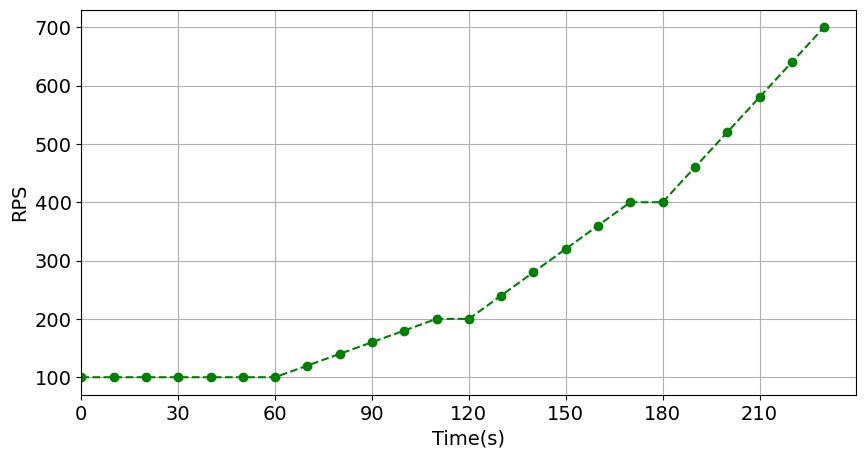
\includegraphics[width=4.2cm]{leejaehong/images/evaluation/linear_test_workload.png}}
    \subfloat[Spike]{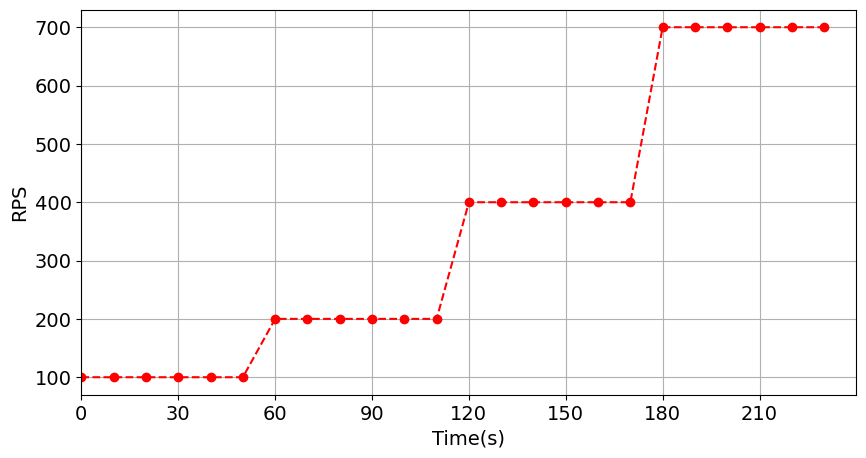
\includegraphics[width=4.2cm]{leejaehong/images/evaluation/spike_test_workload.png}}
    \caption{Test Workloads}
    \label{fig:test_workloads}
\end{figure}

\begin{figure}[ht!]
    \begin{subfigure}{.5\textwidth}
        \centering
        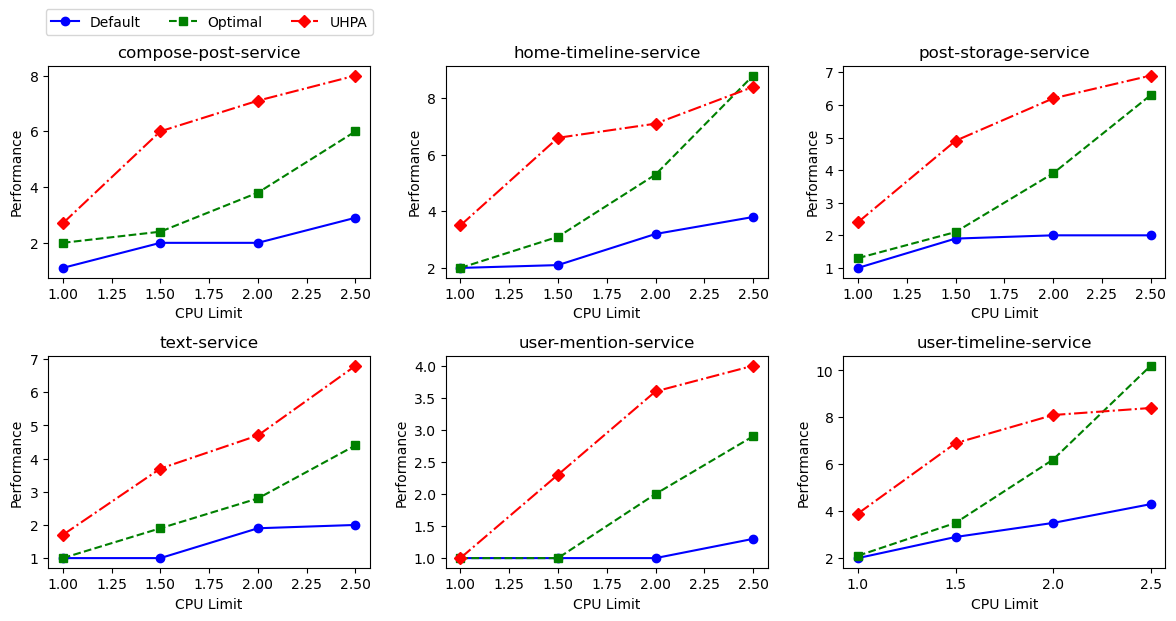
\includegraphics[width=.95\linewidth]{leejaehong/images/evaluation/linear_result.png}
        \caption{Linear}
        \label{fig:num_of_pods_linear}
    \end{subfigure}
    \begin{subfigure}{.5\textwidth}
        \centering
        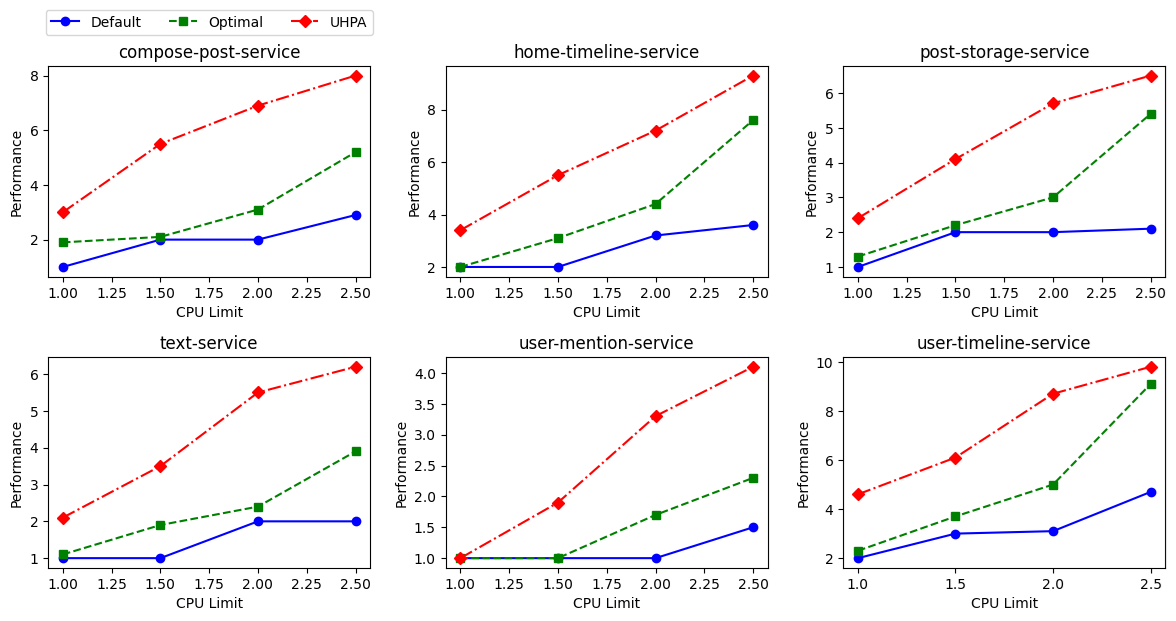
\includegraphics[width=.95\linewidth]{leejaehong/images/evaluation/spike_result.png}
        \caption{Spike}
        \label{fig:num_of_pods_spike}
    \end{subfigure}

    \caption{Number of Pods in According to CPU limit}
    \label{fig:num_of_pods}
\end{figure}



\subsection{System Overhead}
how much this system use resource depending on the number of pods
그림 추가 필요
각 노드에서 pod당 1m cpu만 사용함을 확인



% ----------------------------------------------------------------------------


\section{Conclusion}
problem.

what we found.

what we did.

result with number

% ----------------------------------------------------------------------------


\bibliographystyle{plain}
\bibliography{references}

\vspace{12pt}
\end{document}